\documentclass[12pt]{article}
\usepackage[paperheight=210mm,paperwidth=148mm,top=2cm,bottom=2cm,left=1cm,right=1cm]{geometry}  % A5 paper
\usepackage{background}
\backgroundsetup{
    scale=1,
    opacity=0.1,
    angle=0,
    color=black,
    contents={%
    
\includegraphics[width=\paperwidth]{../../assets/background}
    }
}
%%%%%%%%%%%%%%%%%%%%%%%%%%%%%%%%%%%%%%%%
\usepackage[utf8]{inputenc}
\usepackage[brazil]{babel}
\usepackage{titlesec}
%\usepackage[all]{hypcap}
\usepackage{multirow}
%\usepackage{tikz}
\usepackage{ctable}
%%%%%%%%%%%%%%%%%%%%%%%%%%%%%%%%%%%%%%%%
\renewcommand{\familydefault}{\sfdefault}
% \titleformat{\chapter}[display]
% {\bfseries\LARGE\sffamily}{\chaptertitlename}{10pt}{\LARGE}
% \titlespacing*{\chapter}{0pt}{10pt}{10pt}
% \numberwithin{table}{chapter}


\begin{document}
% Cover
\newgeometry{left=0cm, bottom=0cm, top=0cm, right=0cm}
\thispagestyle{empty}
\noindent  % To remove the unwanted white space.

\includegraphics{../../assets/capa}
\NoBgThispage

\clearpage

\restoregeometry

\newpage

Olá,

esperamos que todos tenha gostado do SciPy Latin America 2016.
Nessa edição contamos com atividades astronômicas para crianças,
um workshop da Software Carpentry,
12 tutoriais e 34 palestras (sendo 18 palestras relâmpago).
% FIXME Incluir o número de horas da trilha para crianças.
Incluindo os eventos sociais tivemos mais de 60h de atividades durante os cinco
dias que compuseram o SciPy Latin America 2016.

% FIXME Corrigir número de participantes para incluir as crianças.
Participaram das atividades mais de 50 pessoas dentre
alunos do ensino fundamental,
alunos de graduação,
alunos de pós-graduação,
professores,
desenvolvedores
e entusiastas.


Att, \\
\indent Ivan Ogasawara \\
\indent Presidente da SciPy Latin America 2016


\newpage

\section*{Programa}

O SciPy Latin America 2016 ocorreu na cidade de Florianópolis, Santa Catarina,
Brasil. A cidade localiza-se em uma ilha.

\noindent  % To remove the unwanted white space.
\begin{figure}[!htb]
\center
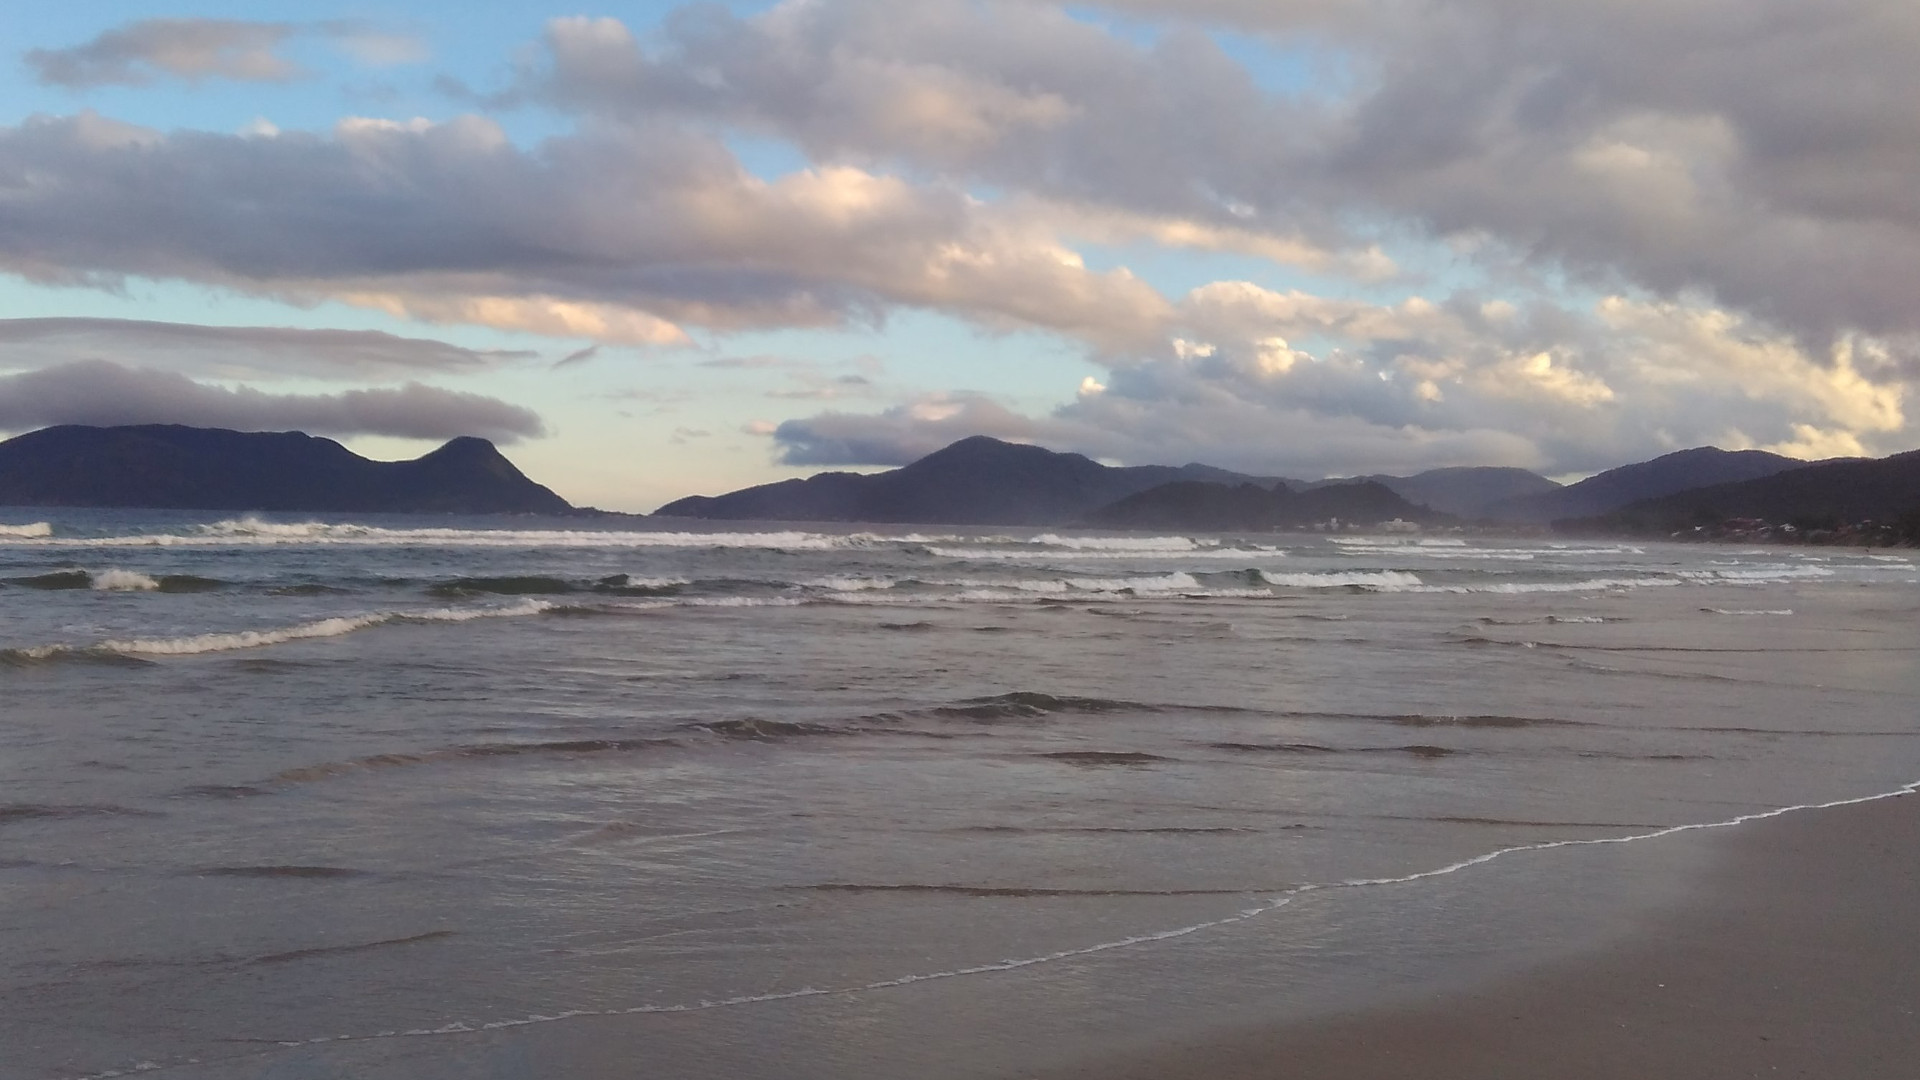
\includegraphics[height=.3\textheight]{venue-beach.jpg}
\caption{FIXME}
\end{figure}

\subsection*{Workshop}

O workshop da Software Carpentry aconteceu no Centro de Informática e Automação
do Estado de Santa Catarina S.A.

\noindent  % To remove the unwanted white space.
\begin{figure}[!htb]
\center
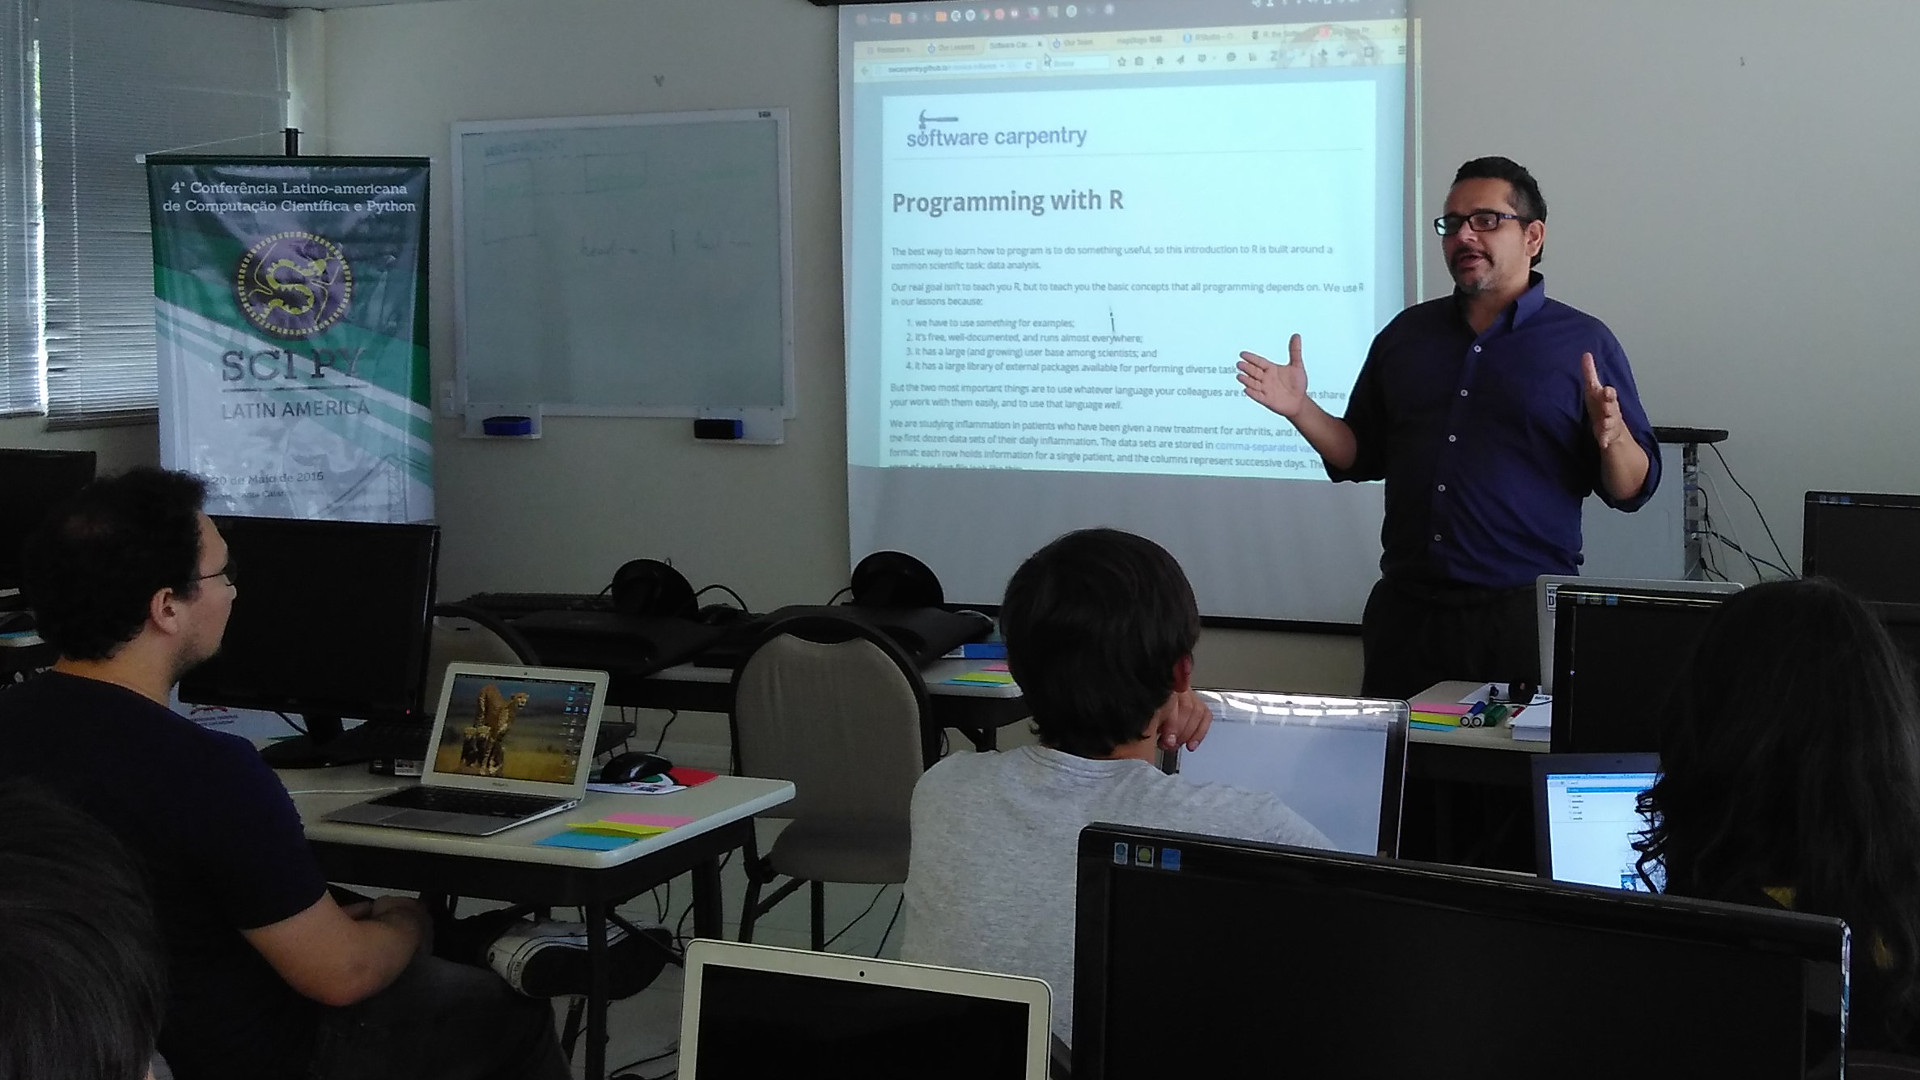
\includegraphics[height=.3\textheight]{swc-francisco.jpg}
\caption{FIXME}
\end{figure}

Os instrutores no workshop foram Raniere Silva e Francisco Palm,
ambos instrutores certificados da Software Carpentry.
No workshop foi apresentado o terminal UNIX, controle de versão com Git,
compartilhamento de trabalho com o GitLab e programação com R.

\noindent  % To remove the unwanted white space.
\begin{figure}[!htb]
\center
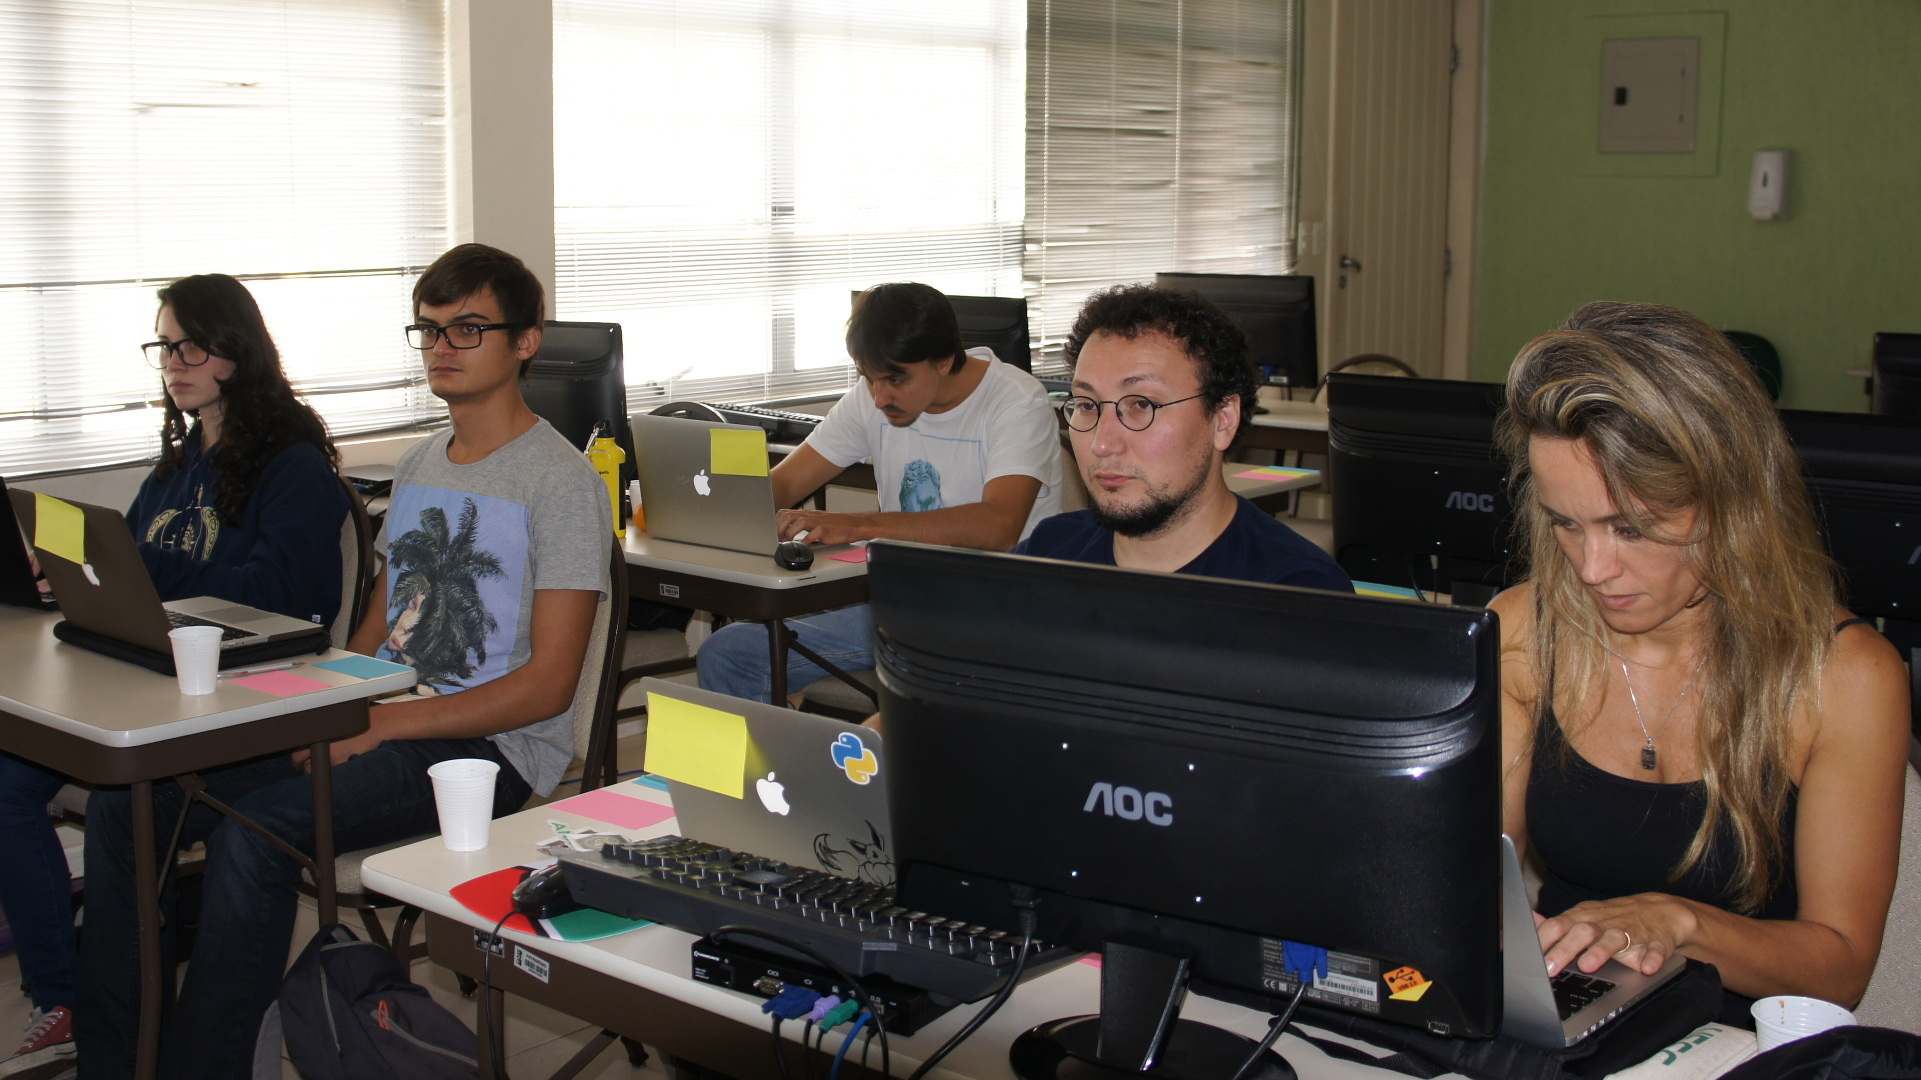
\includegraphics[height=.3\textheight]{swc-students.jpg}
\caption{FIXME}
\end{figure}

Sete dos vinte alunos matriculados compareceram no workshop.
Alguns não participaram de todo o workshop porque foram em um dos tutoriais que
acontecia no mesmo período ou tinham outras obrigações.

O feedback dos alunos foi bastante positivo. Eles gostaram do workshop
e reclamaram que a Universidade de Santa Catarina não oferece mais workshops
como os oferecidos pela Software Carpentry.

\subsection*{Tutoriais}



\noindent  % To remove the unwanted white space.
\begin{figure}[!htb]
\center
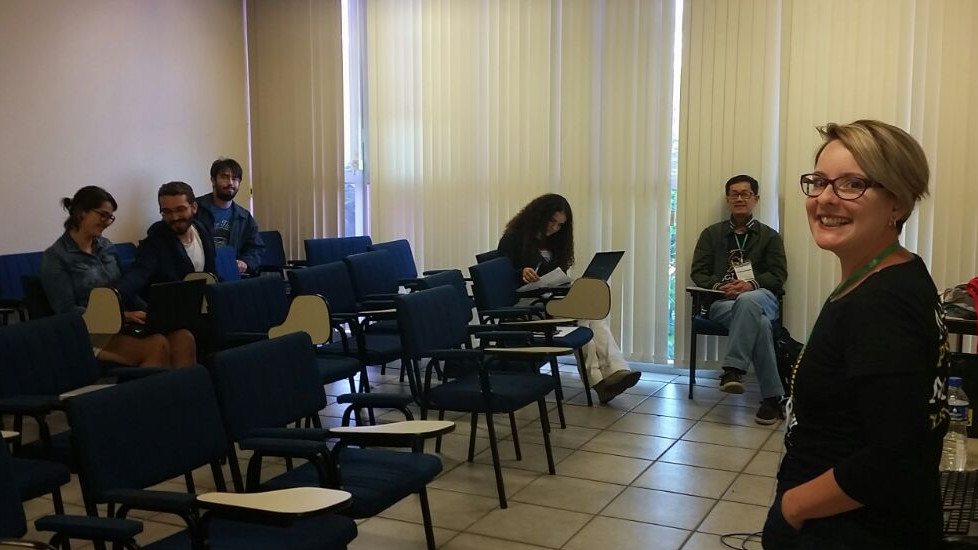
\includegraphics[height=.3\textheight]{tutorial-latex.jpg}
\caption{Fernando Masanori e seu slide ``I Love PyLadies''.}
\end{figure}

\noindent  % To remove the unwanted white space.
\begin{figure}[!htb]
\center
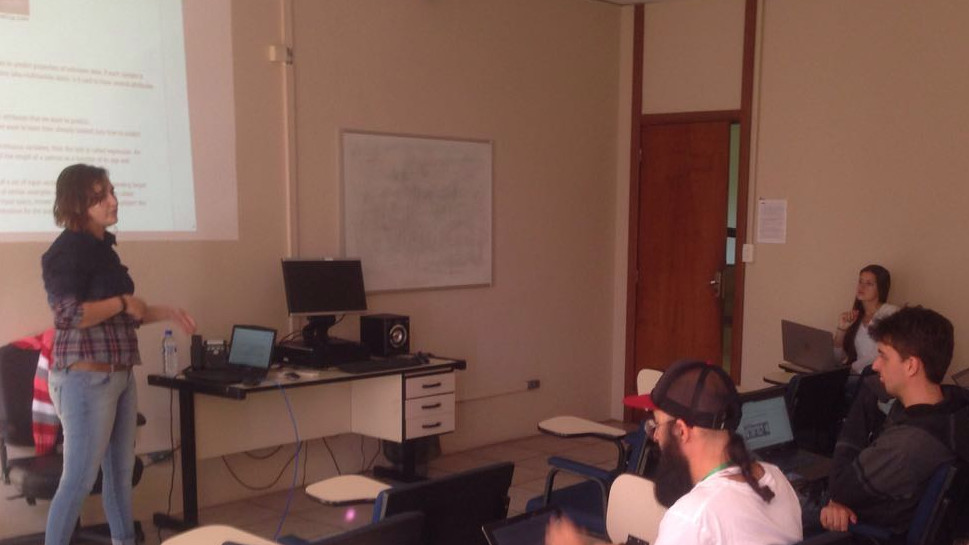
\includegraphics[height=.3\textheight]{tutorial-pyopencl.jpg}
\caption{Fernando Masanori e seu slide ``I Love PyLadies''.}
\end{figure}

\noindent  % To remove the unwanted white space.
\begin{figure}[!htb]
\center
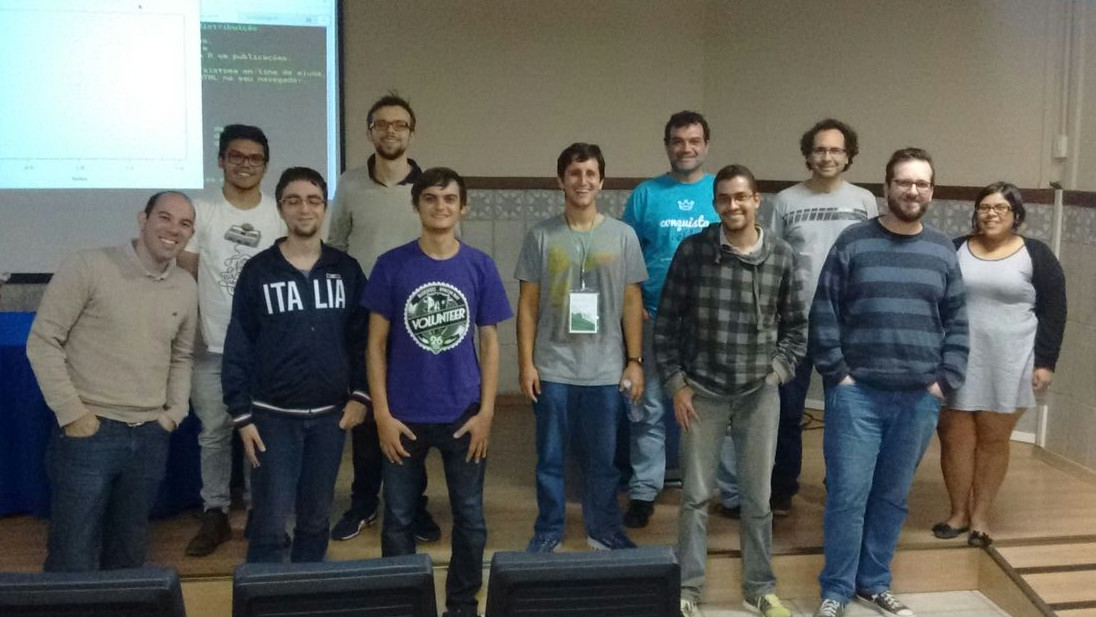
\includegraphics[height=.3\textheight]{tutorial-rpy.jpg}
\caption{Fernando Masanori e seu slide ``I Love PyLadies''.}
\end{figure}

\subsection*{Palestras}

Durante o evento ocorreram 16 palestras e 18 palestras relâmpagos.

\begin{figure}[!htb]
\center
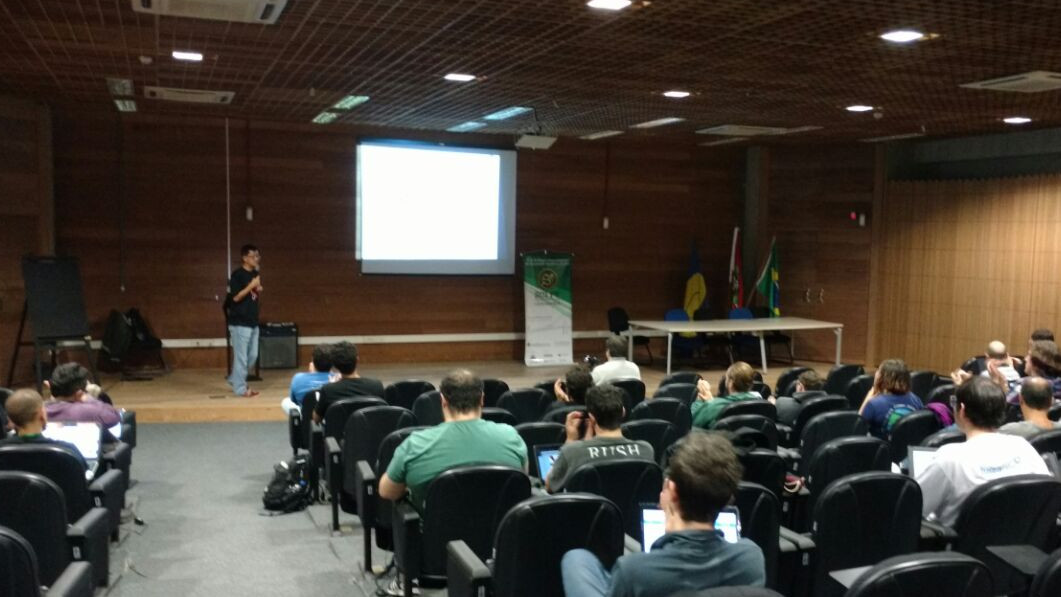
\includegraphics[height=.3\textheight]{talks-full.jpg}
\caption{Auditório durante as palestras.}
\end{figure}

As palestras cobriram vários domínios da ciência, incluindo
oceanografia,
genética,
fármacos,
matemática,
estatística.

\begin{figure}[!htb]
\center
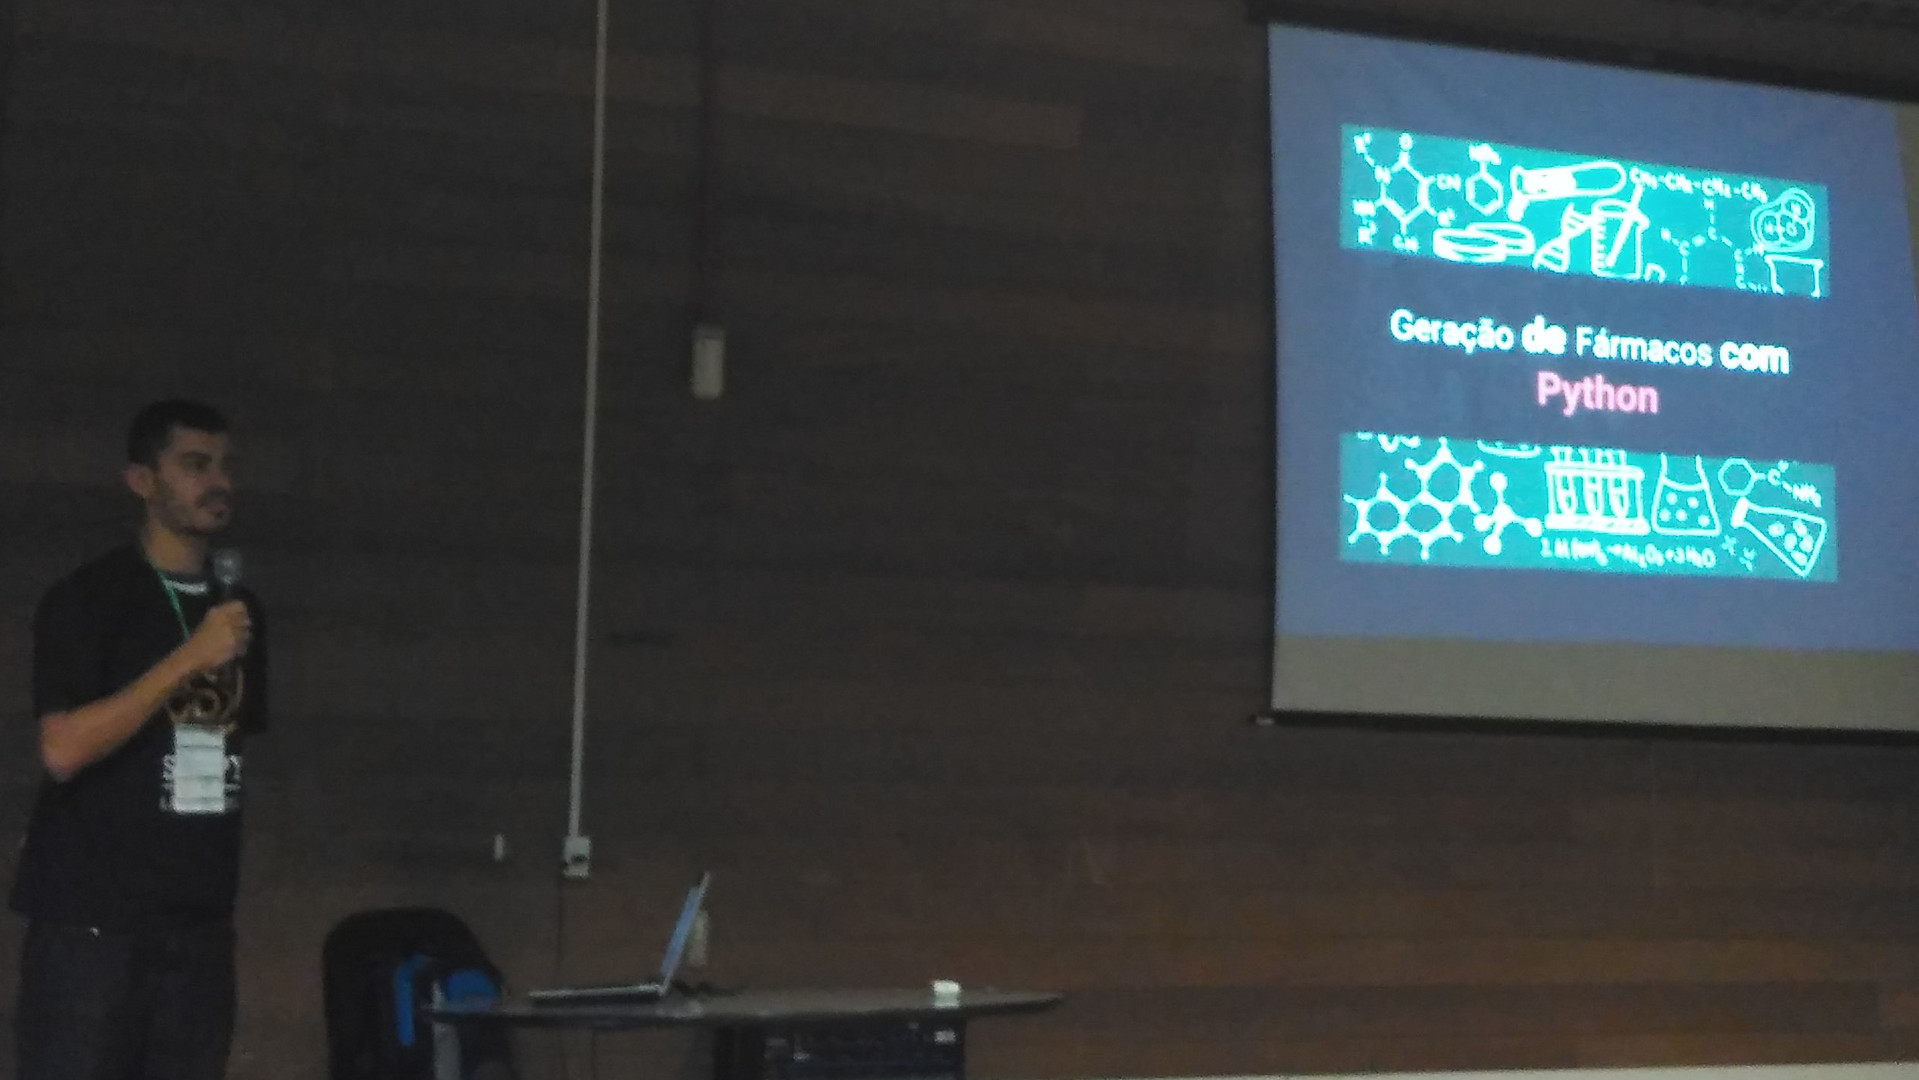
\includegraphics[height=.3\textheight]{talks-drugs.jpg}
% FIXME Colocar nome completo do Mario
\caption{Mario falando sobre geração de fármacos.}
\end{figure}

Também tivemos palestras técnicas relacionadas com ferramentas utilizadas em
computação científica. Dentre essas palestras destacaram-se ``The numba
library'' de Edison Gustavo Muenz, ``Conda-forge and the future of the
Scientific Python package'' de Filipe Fernandes e ``Interactive Data
Visualization in the Browser with Bokeh'' de Bryan Van de Ven.

\begin{figure}[!htb]
\center
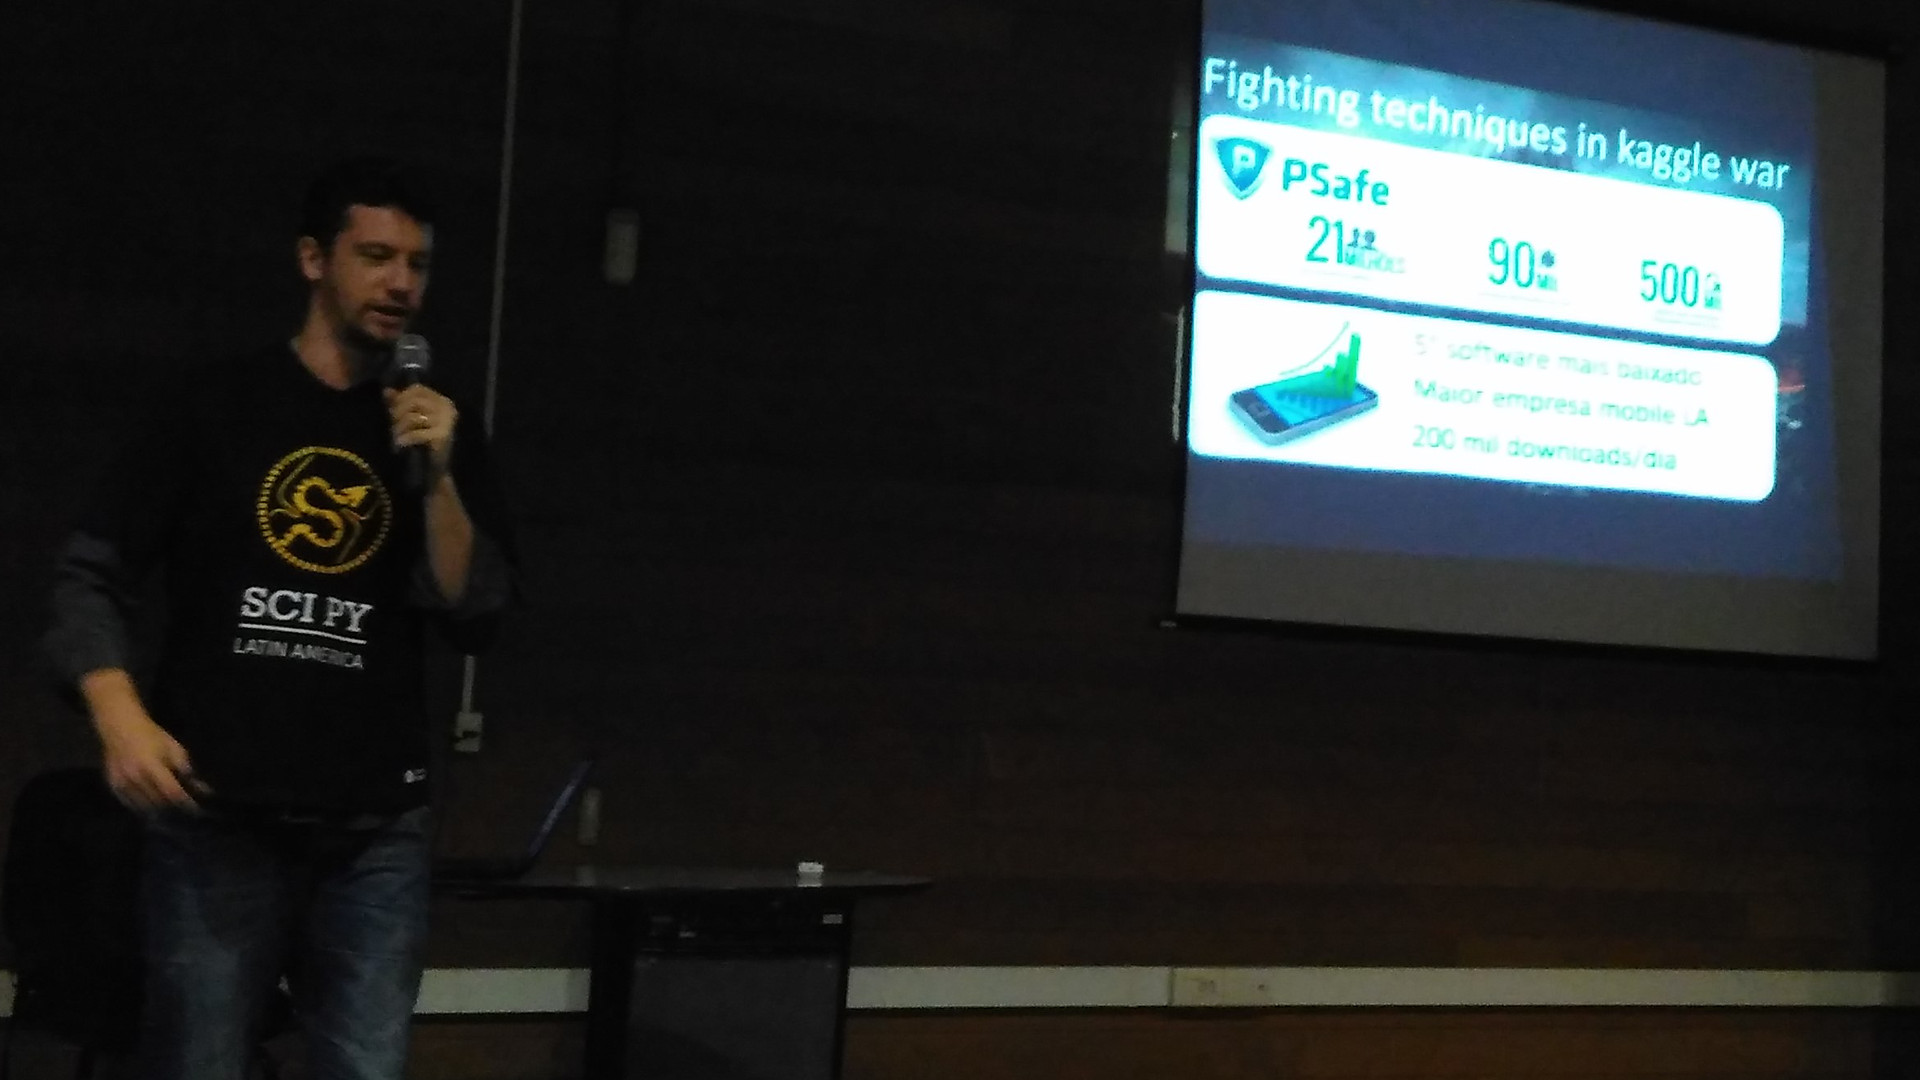
\includegraphics[height=.3\textheight]{talks-kaggle.jpg}
% FIXME Colocar nome do palestrante.
\caption{falando sobre Kaggle.}
\end{figure}

Além das palestras científicas e técnicas também ocorreram palestras voltadas
ao desenvolvimento de comunidades. Destacaram-se ``import community'' por
Fernando Masanori e ``Estudo de caso: Software Sustainability Institute'' por
Raniere Silva.

\begin{figure}[!htb]
\center
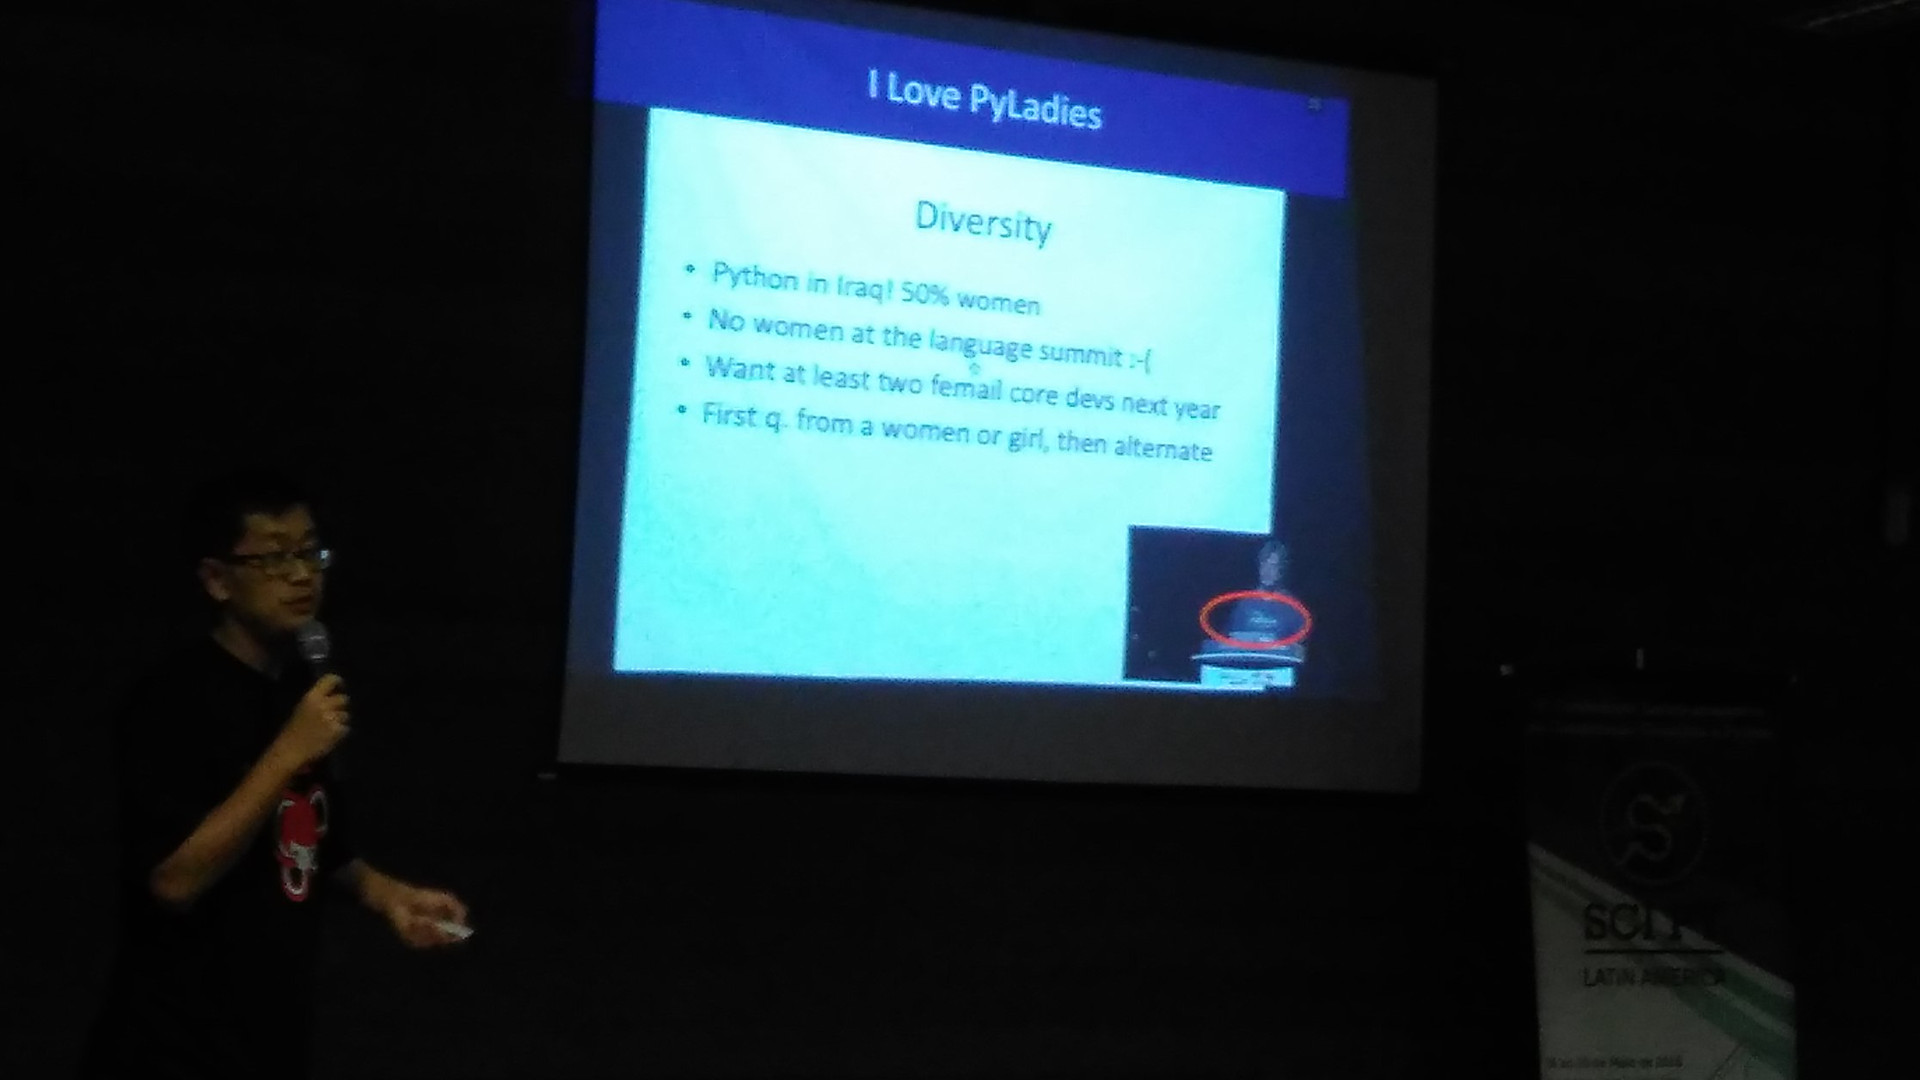
\includegraphics[height=.3\textheight]{talks-pyladies.jpg}
\caption{Fernando Masanori e seu slide ``I Love PyLadies''.}
\end{figure}

Nas palestras relâmpagos vários participantes proferiram suas primeiras
palestras. Esperamos revê-los novamente na Python Brasil 2016, SciPy Latin
America 2017 e outras conferências ao redor do mundo.

\begin{figure}[!htb]
\center
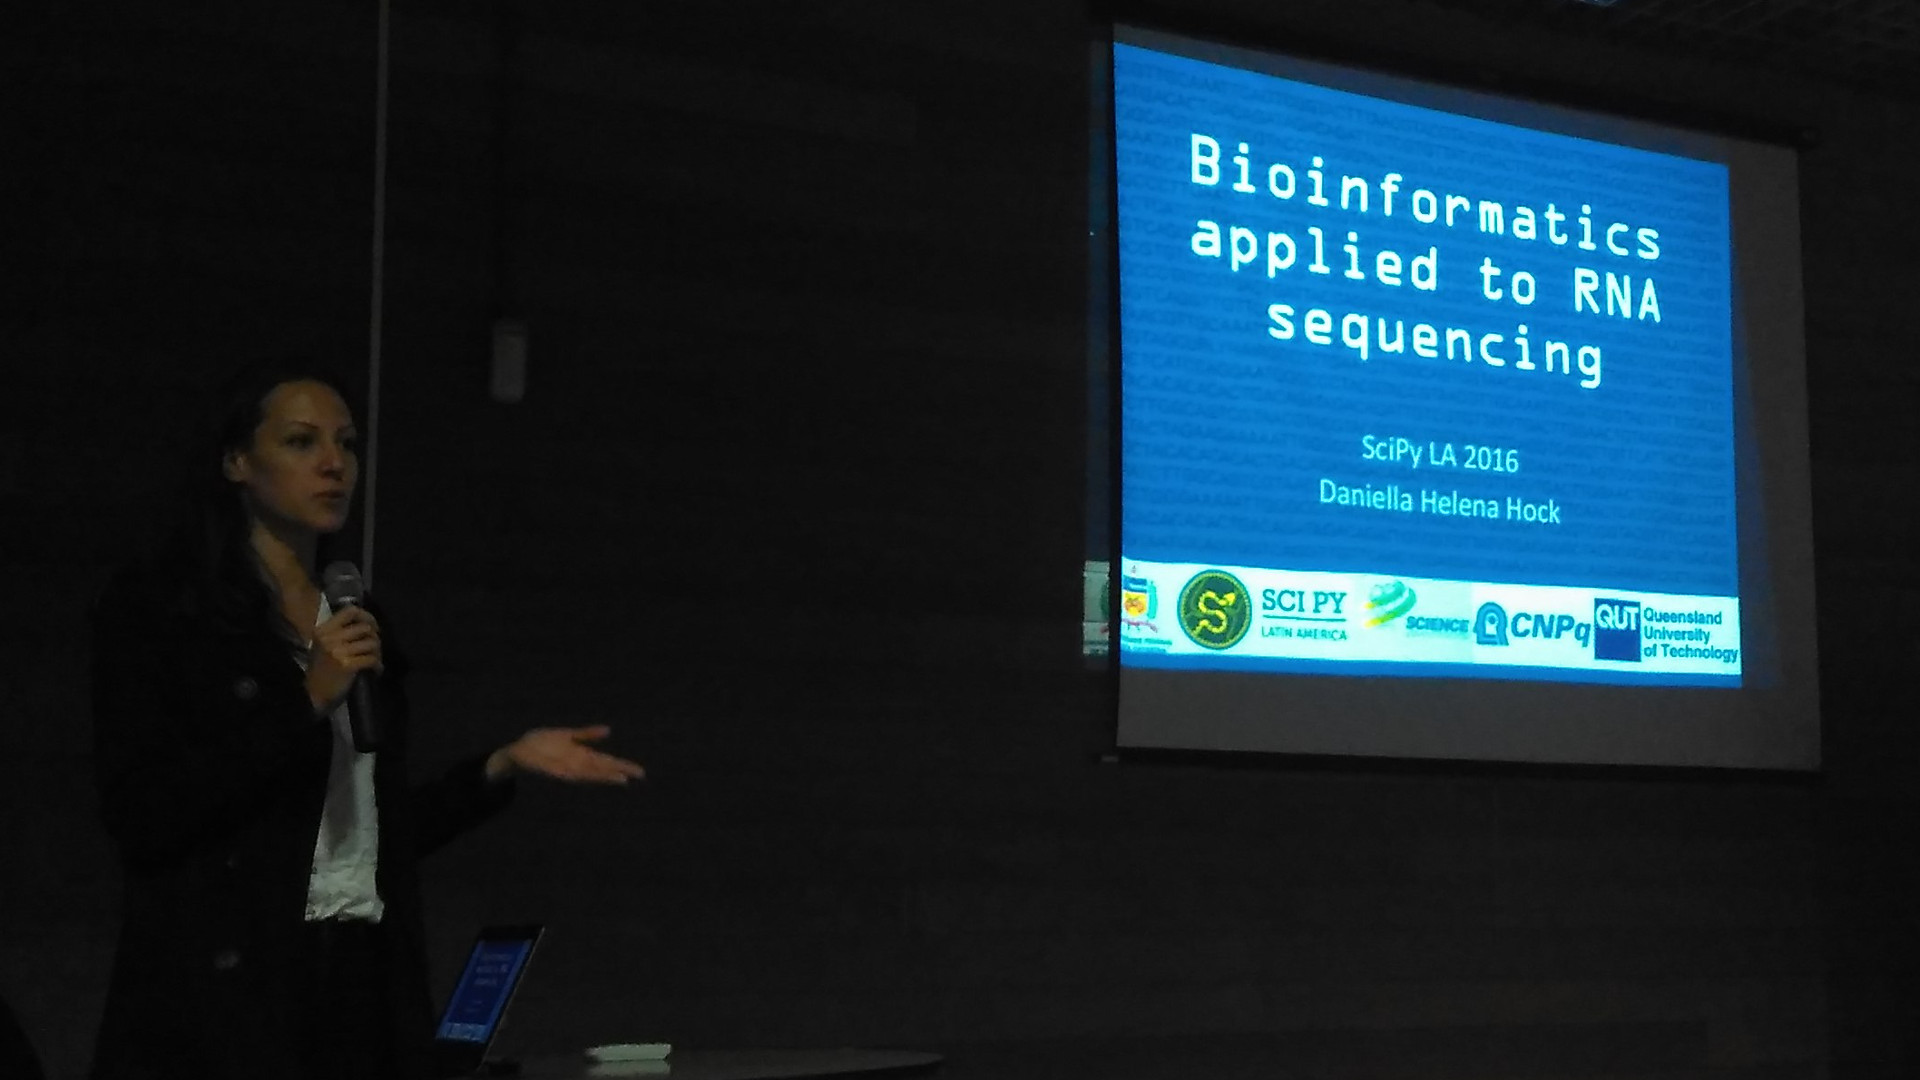
\includegraphics[height=.3\textheight]{talks-rna.jpg}
\caption{Daniella em sua apresentação sobre sequências e RNA.}
\end{figure}

Vários participantes disseram que a coleção de palestras estava excelente.

\subsection*{Eventos sociais}

Durante o SciPy Latin America ocorreram vários eventos sociais para os
participantes. Durante todo o evento estiveram disponíveis aos participantes uma
coleção de chás e chocolates que foram complementados com algumas frutas e doces
locais.

\begin{figure}[!htb]
\center
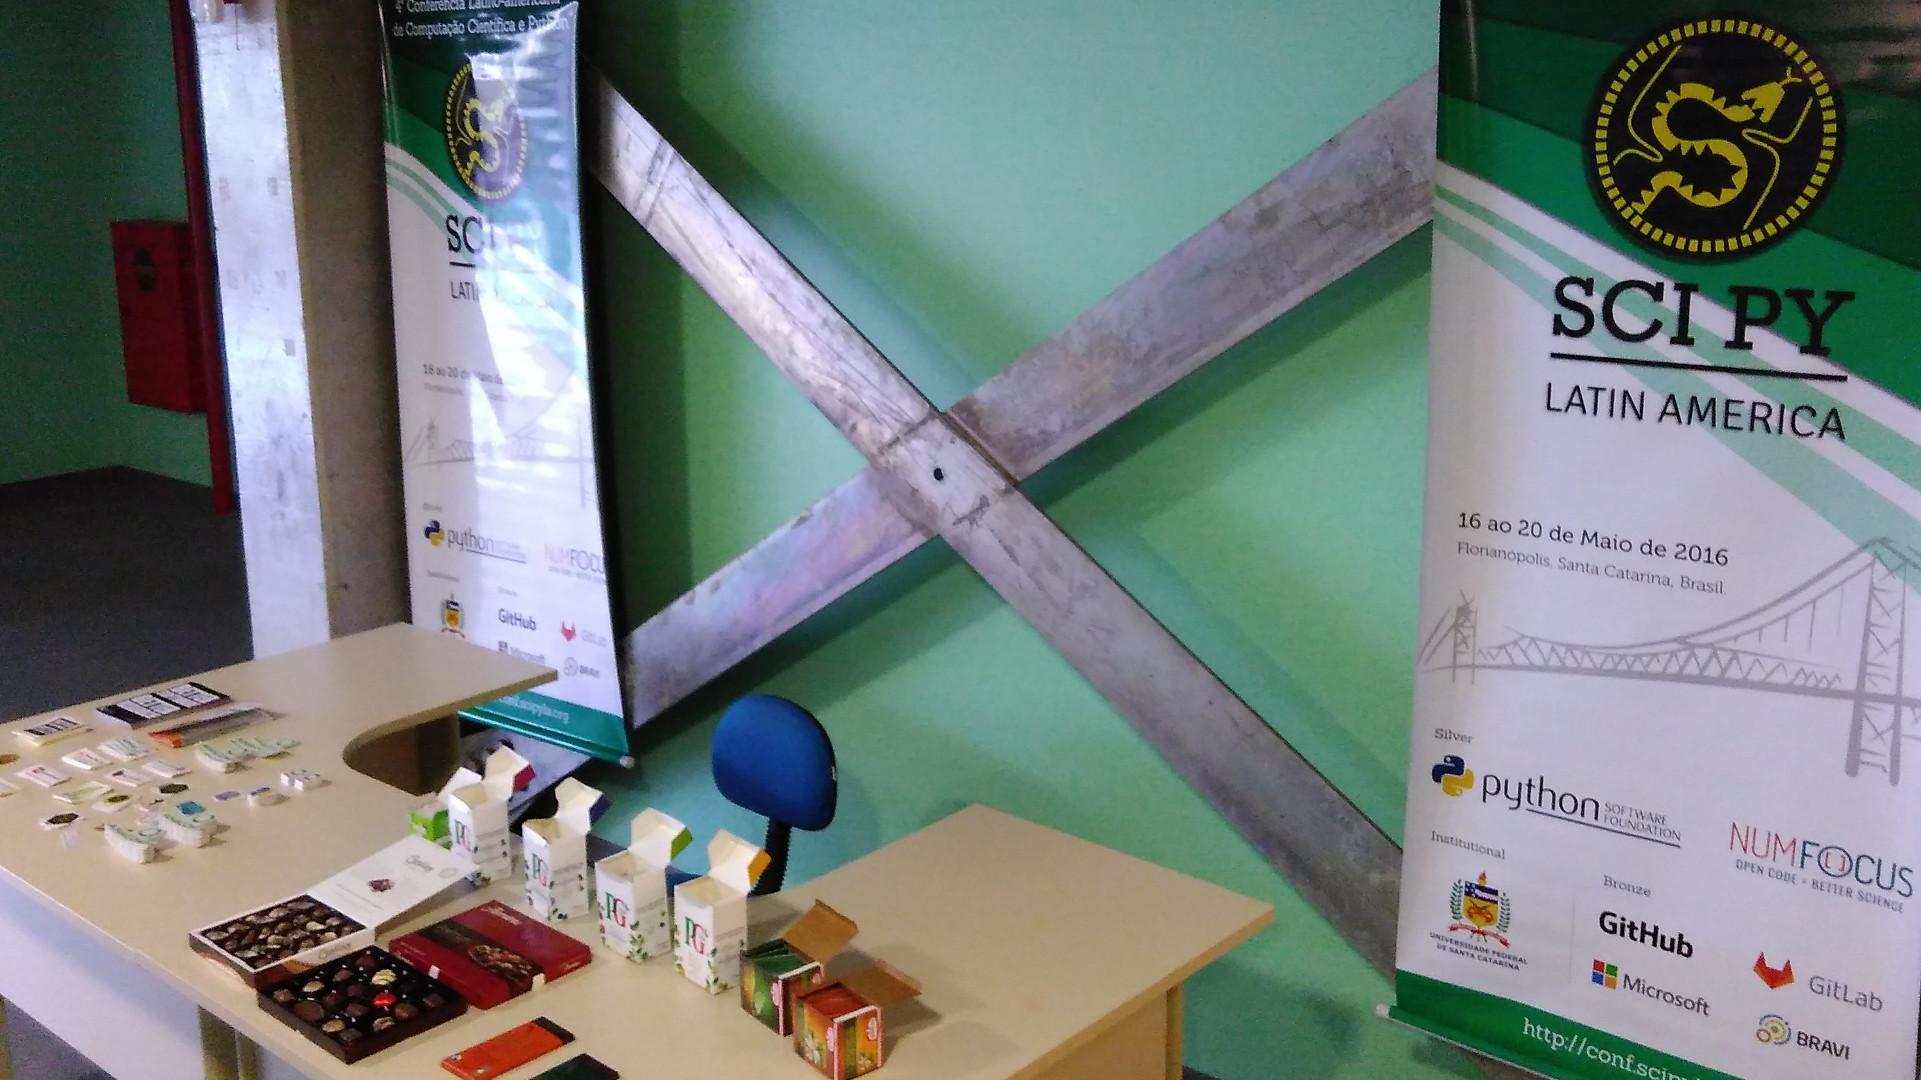
\includegraphics[height=.3\textheight]{social-break.jpg}
\caption{FIXME}
\end{figure}

Florianópolis é famosa pelas várias cervejarias artesanais locais.
Os participantes visitaram algumas dessas cervejarias durante os happy hours.
Todas os lugares escolhidos para os happy hours ofereciam opções para
vegetarianos e estes gostaram bastante das opções existentes nos cardápios.

\begin{figure}[!htb]
\center
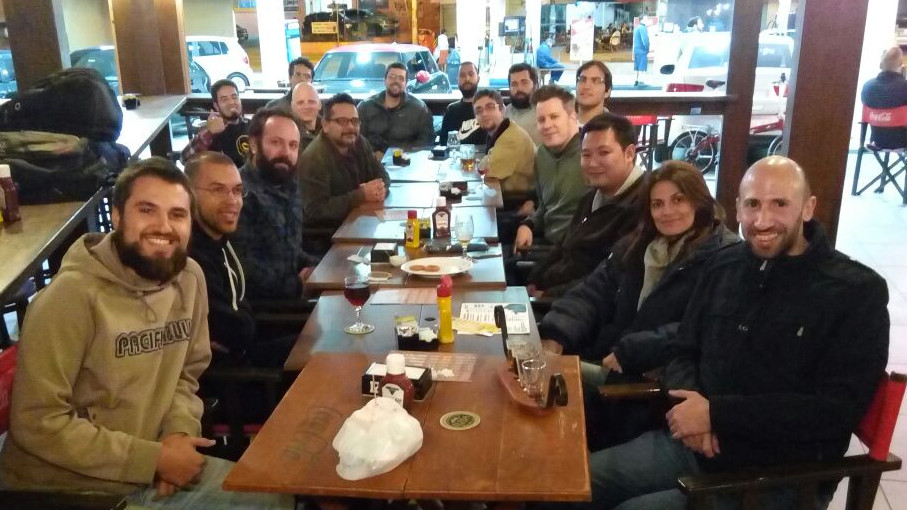
\includegraphics[height=.3\textheight]{social-viking.jpg}
\caption{FIXME}
\end{figure}

Um dos bares que visitamos tem paredões para escalada
e alguns dos participantes se aventuraram ao praticar bouldering.
Esse bar possui um ambiente bem familiar e descontraído
o que ajudou os participantes a aproveitarem a noite.

\begin{figure}[!htb]
\center
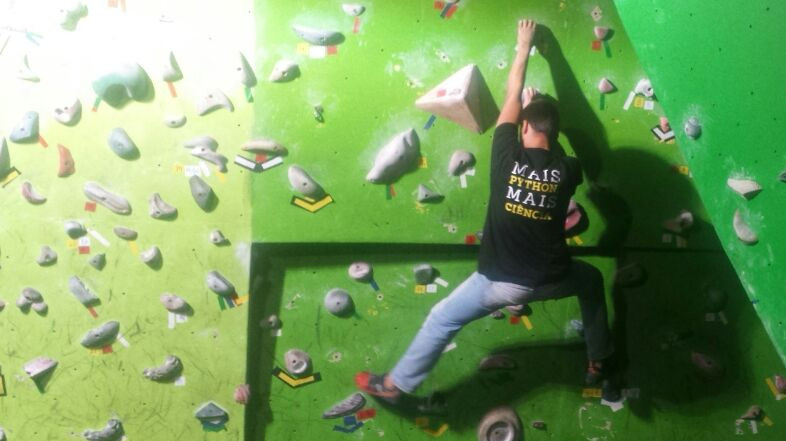
\includegraphics[height=.3\textheight]{python-escala.jpg}
\caption{FIXME}
\end{figure}

Na noite do dia 19, o Observatório da Universidade Federal de Santa Catarina
promoveu uma visita guiada ao seu espaço e observação do céu.
Embora estivesse frio, todos os participantes gostaram de ver a Lua, Marte e
alguns estrelas por meio dos telescópios.
Os astrônomos que participavam da conferência adoraram a visita guiada.

\begin{figure}[!htb]
\center
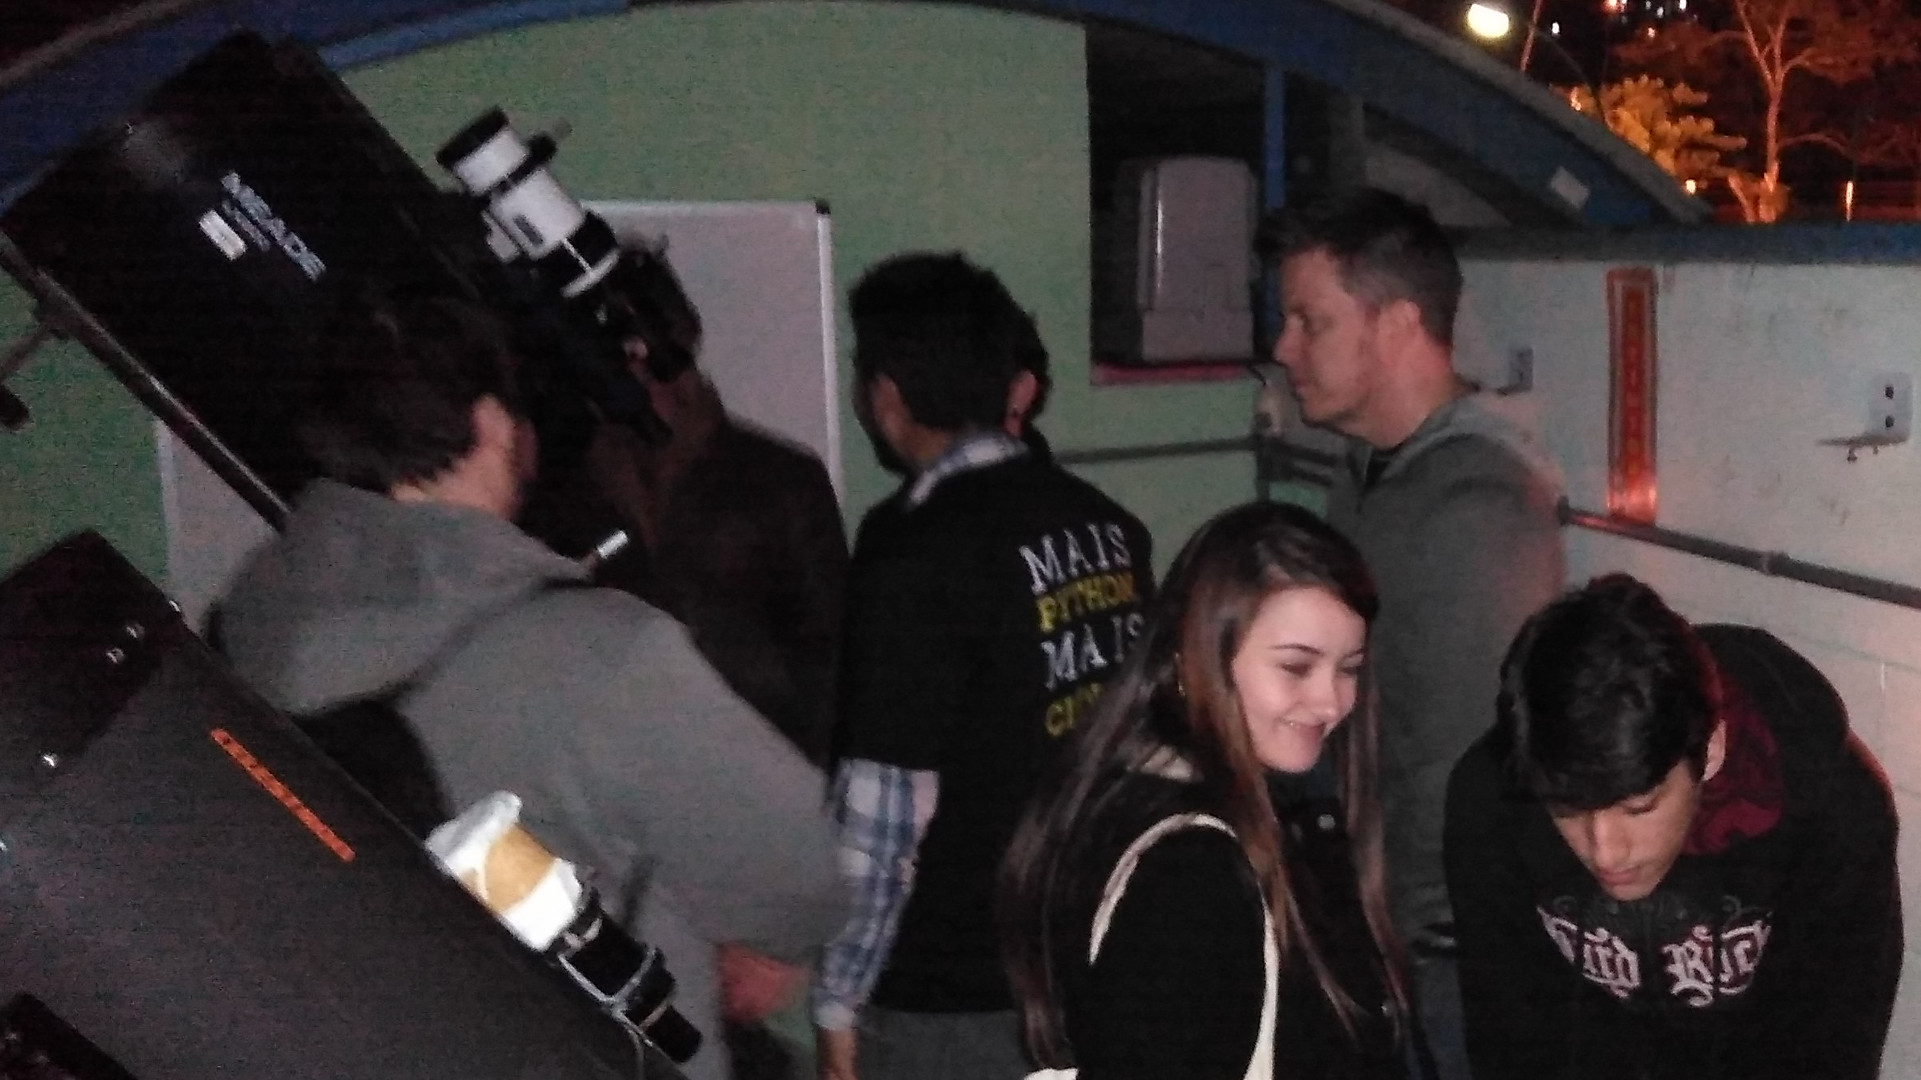
\includegraphics[height=.3\textheight]{social-astro.jpg}
\caption{FIXME}
\end{figure}

Alguns participantes levaram seus filhos para participar da visita guiada ao
Observatório.

\begin{figure}[!htb]
\center
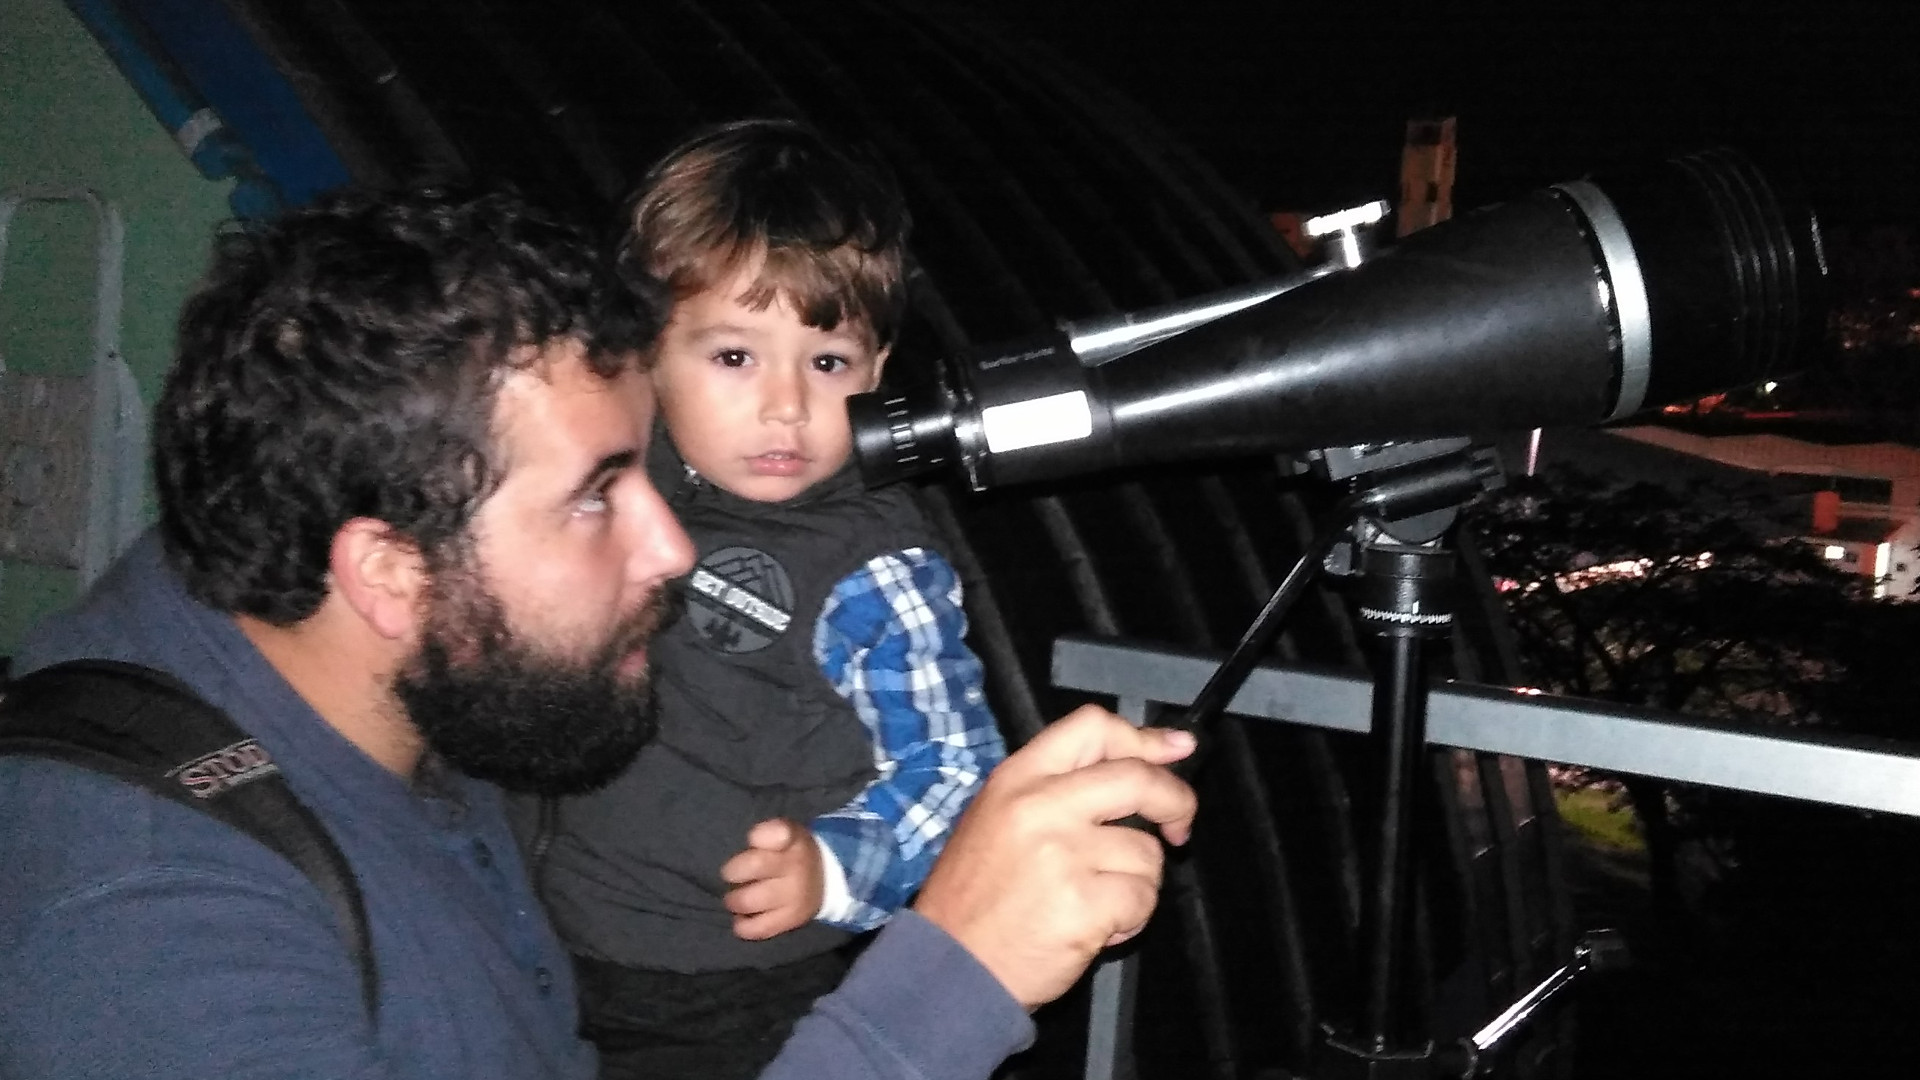
\includegraphics[height=.3\textheight]{social-family.jpg}
\caption{FIXME}
\end{figure}

\newpage

\section*{Público}

\begin{figure}[!htb]
\center
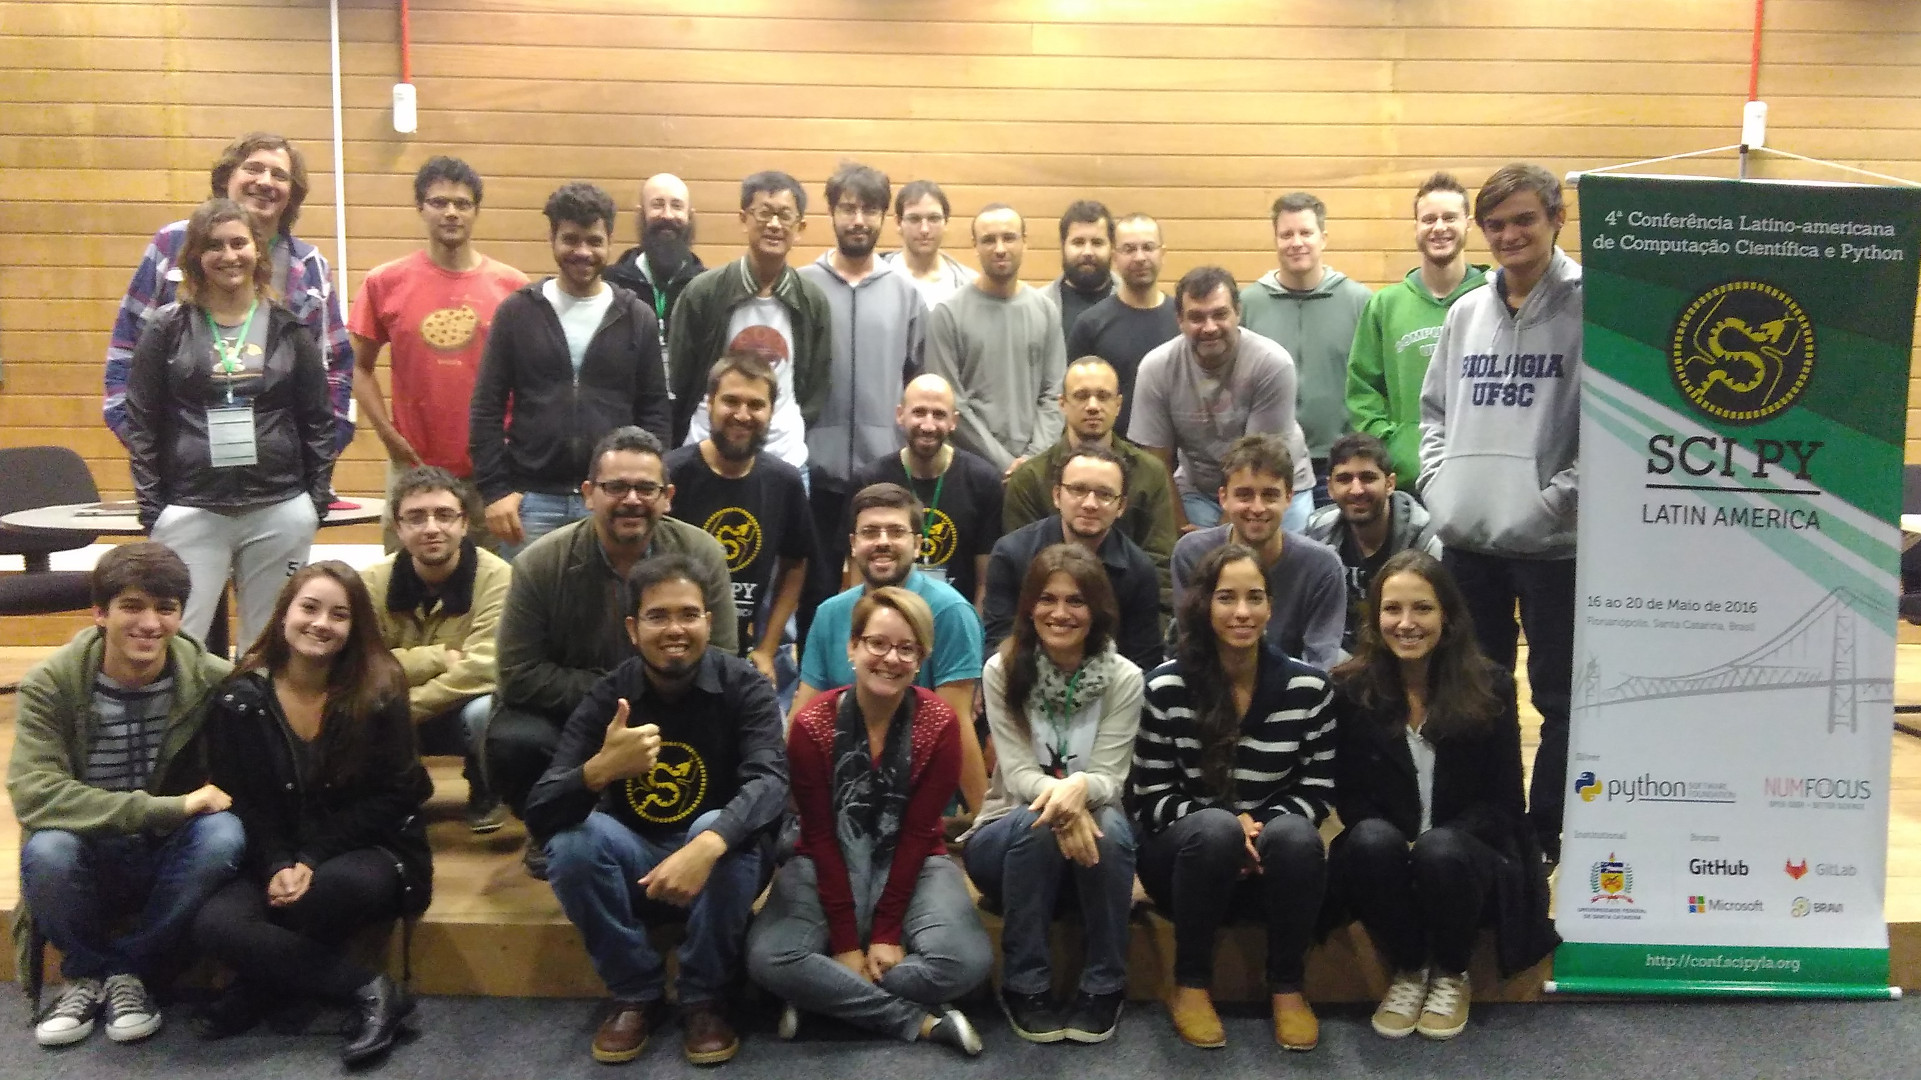
\includegraphics[height=.3\textheight]{group.jpg}
\caption{FIXME}
\end{figure}

O SciPy Latin America 2016 recebeu mais de 160 inscritos paras as palestras e
uma média de 20 inscritos em cada um dos tutoriais que foram oferecidos.
Nas palestras tivemos um público médio de 50 pessoas. Nos tutoriais o público
variou bastante.

As inscrições nos tutoriais e palestras eram gratuitos. Embora a taxa de
ausentes seja alta ela está dentro de valores relatados por outros eventos
similares.

Para os próximos eventos estamos planejando cobrar inscrições com o objetivo de
aumentar a presença.

O número de mulheres no evento foi de 10\%. Uma taxa baixa mas que está na média
para eventos do tipo.

\newpage

\section*{Repercussão}

No Brasil, o uso do Twitter e comentários sobre o evento nas demais redes
sociais como Facebook e Instagram não é muito comum. Mesmo assim tivemos alguns
comentários positivos no Twitter.

\begin{figure}[!htb]
\center
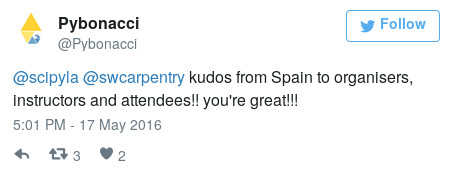
\includegraphics[height=.3\textheight]{tweet-kudos.jpg}
\caption{Usuário de Python na Espanha parabenizando o SciPy Latin America 2016.}
\end{figure}

Aqueles que acompanharam a hashtag \#SciPyLA2016 no Twitter ou a página do
evento no Facebook foram informados continuamente sobre as palestras e demais
atividades que estavam ocorrendo no evento.

\begin{figure}[!htb]
\center
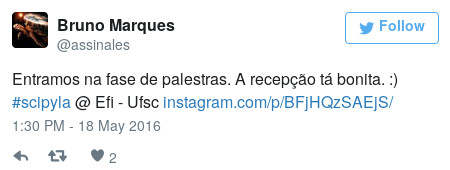
\includegraphics[height=.3\textheight]{tweet-recepcao.jpg}
\caption{Participante dizendo que a recepção do SciPy Latin America 2016 está
bonita.}
\end{figure}

\begin{figure}[!htb]
\center
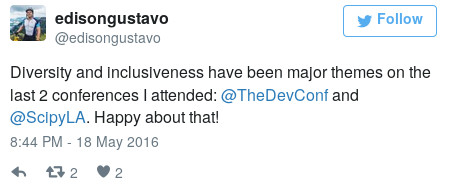
\includegraphics[height=.3\textheight]{tweet-diversidade.jpg}
\caption{Participante dizendo estar feliz pelo SciPy Latin America 2016 falar
sobre diversidade.}
\end{figure}

\newpage

\section*{Resultados}

\newpage

\section*{Finanças}

\newpage

\section*{Próxima edição}

\begin{figure}[!htb]
\center
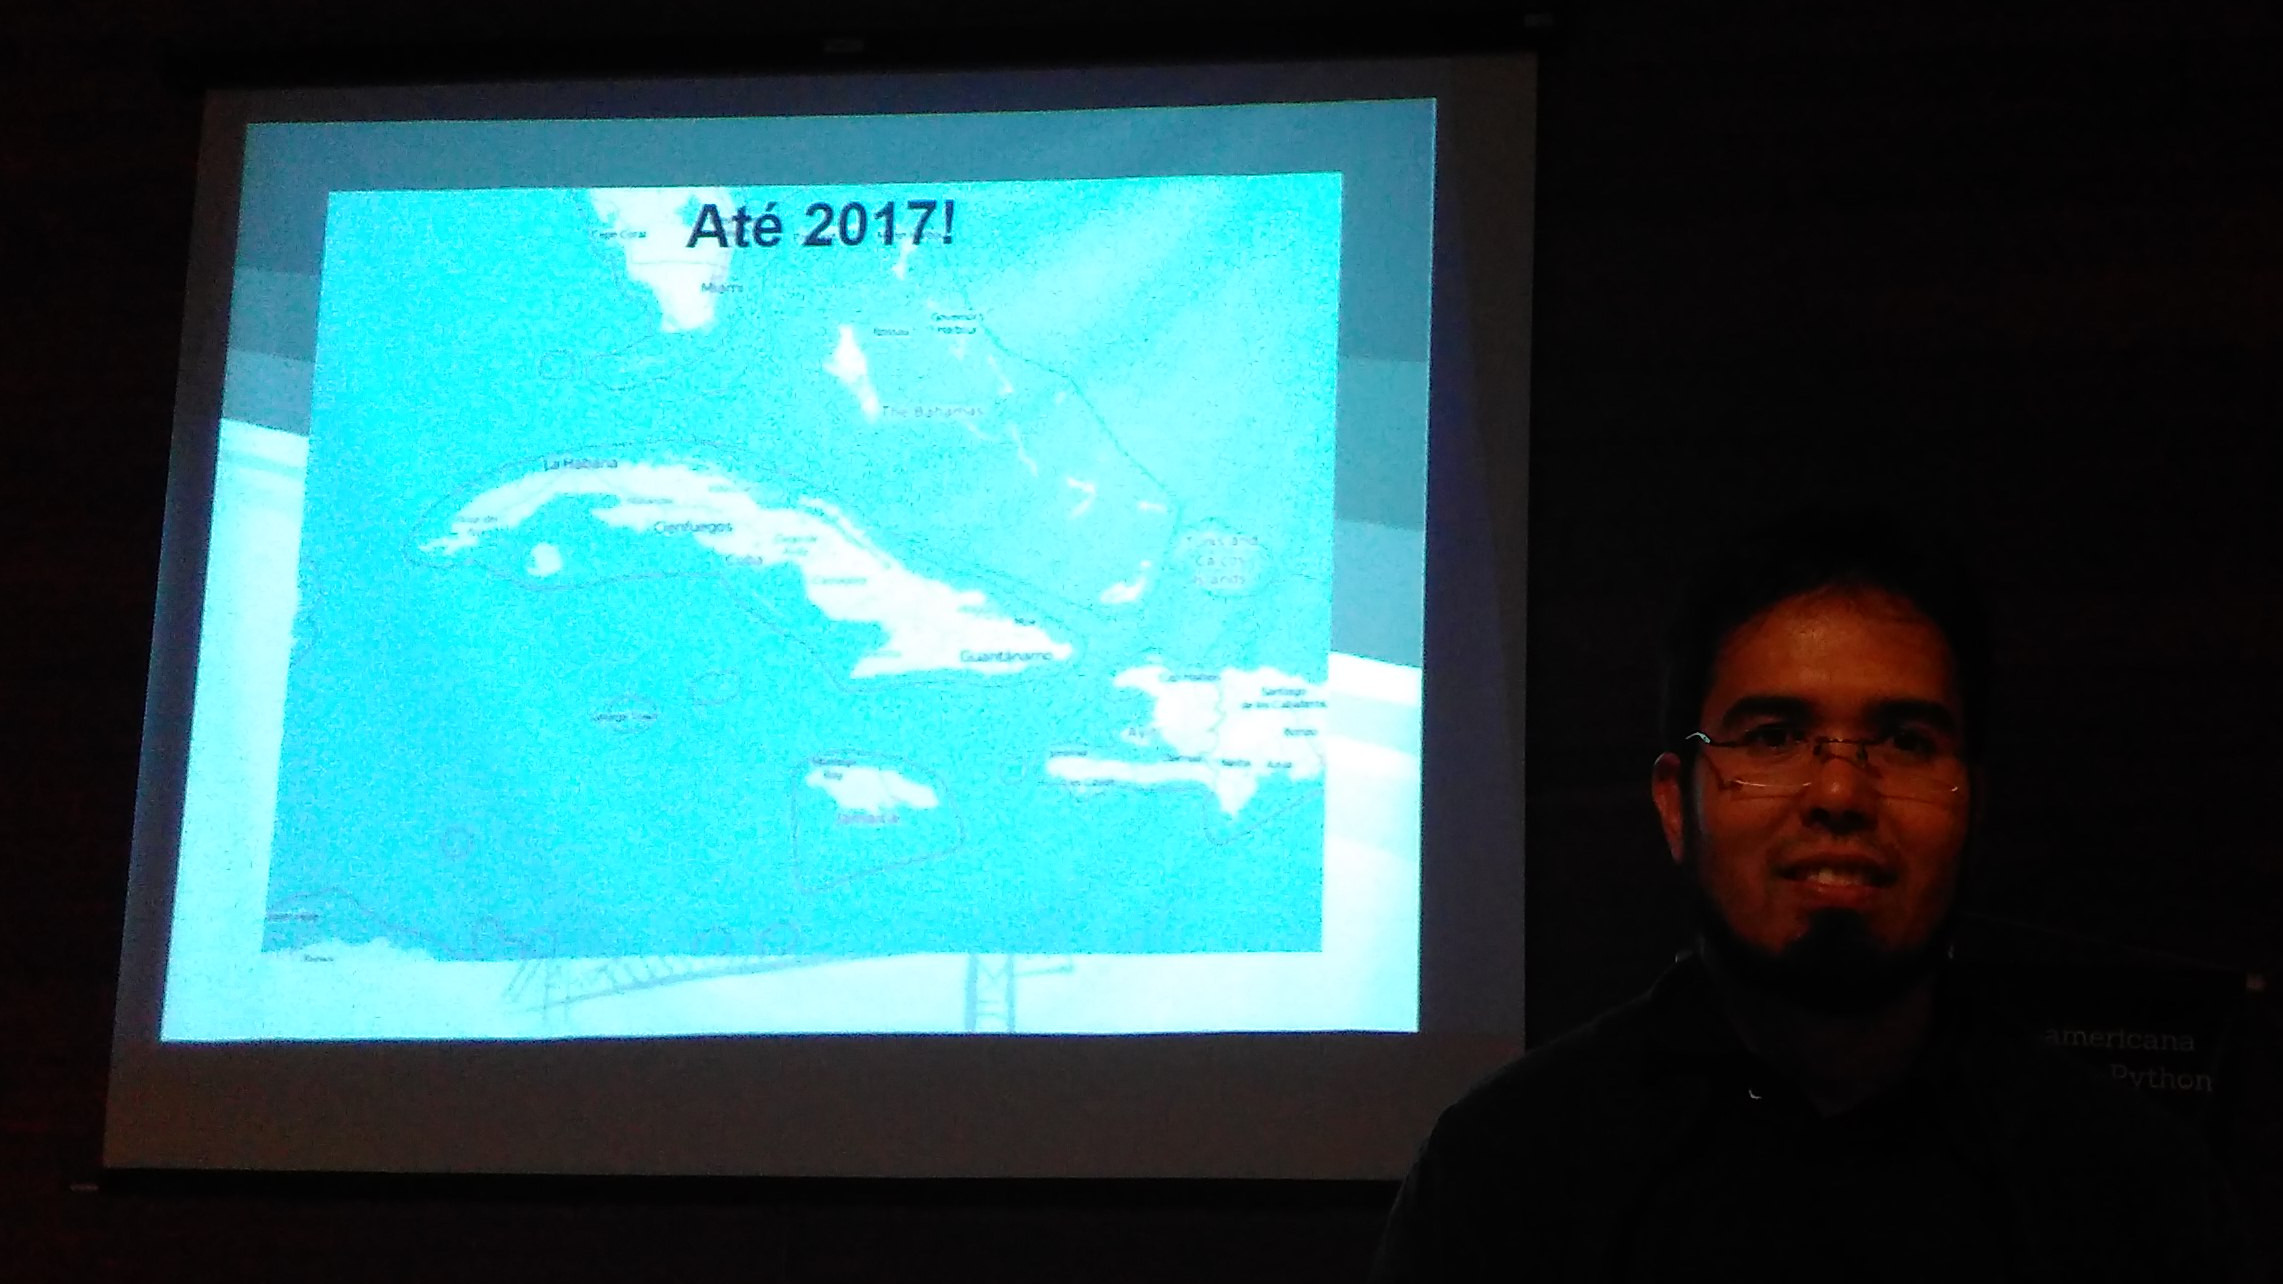
\includegraphics[height=.3\textheight]{2017.jpg}
\caption{FIXME}
\end{figure}

\newpage

% Cover
\newgeometry{left=0cm, bottom=0cm, top=0cm, right=0cm}
\thispagestyle{empty}
\noindent  % To remove the unwanted white space.

\includegraphics{../../assets/contra-capa}
\NoBgThispage


\end{document}
